% Sensors submission manuscript, 3 August 2026
% Official MDPI LaTeX class and files downloaded from:
% https://mdpi-res.com/data/MDPI_template.zip?v=20260313
\documentclass[sensors,article,submit,pdftex,moreauthors]{Definitions/mdpi}

% MDPI internal commands -- retained from the official template.
\firstpage{1}
\makeatletter
\setcounter{page}{\@firstpage}
\makeatother
\pubvolume{1}
\issuenum{1}
\articlenumber{0}
\pubyear{2026}
\copyrightyear{2026}
\datereceived{ }
\daterevised{ }
\dateaccepted{ }
\datepublished{ }
\hreflink{https://doi.org/}

\setlength{\emergencystretch}{2em}
\setlength{\headheight}{25pt}

% Review aid: keep enabled while placing figures and tables; disable for submission.
\newif\ifhighlightfloats
\highlightfloatsfalse
\definecolor{floatreviewblue}{RGB}{0,82,204}
\providecommand{\figref}[1]{}
\providecommand{\tabref}[1]{}
\ifhighlightfloats
  \AtBeginEnvironment{figure}{\color{floatreviewblue}}
  \AtBeginEnvironment{figure*}{\color{floatreviewblue}}
  \AtBeginEnvironment{table}{\color{floatreviewblue}}
  \AtBeginEnvironment{table*}{\color{floatreviewblue}}
  \renewcommand{\figref}[1]{\textcolor{floatreviewblue}{Fig.~\ref{#1}}}
  \renewcommand{\tabref}[1]{\textcolor{floatreviewblue}{Table~\ref{#1}}}
  \newcommand{\reviewcaption}[1]{\caption{\textcolor{floatreviewblue}{#1}}}
\else
  \renewcommand{\figref}[1]{Fig.~\ref{#1}}
  \renewcommand{\tabref}[1]{Table~\ref{#1}}
  \newcommand{\reviewcaption}[1]{\caption{#1}}
\fi
\newcommand{\reviewplaceholder}[2][0.12\textheight]{%
  \fcolorbox{floatreviewblue}{blue!4}{%
    \parbox[c][#1][c]{\dimexpr\linewidth-2\fboxsep-2\fboxrule\relax}{%
      \centering\color{floatreviewblue}\bfseries #2}}}

\Title{Expert-Consistency-Guided Proposal Refinement for 3D Object Detection
from Sparse Radar Point Clouds}
\TitleCitation{Expert-Consistency-Guided Proposal Refinement for 3D Object
Detection from Sparse Radar Point Clouds}

\Author{Zixuan Liu $^{1}$ and Wei Xiong $^{2,3,*}$}
\AuthorNames{Zixuan Liu and Wei Xiong}
\AuthorCitation{Liu, Z.; Xiong, W.}

\address{%
$^{1}$ \quad Detroit Green Technology Institute, Hubei University of
Technology, Wuhan 430068, China\\
$^{2}$ \quad School of Electrical and Electronic Engineering, Hubei University
of Technology, Wuhan 430068, China\\
$^{3}$ \quad Department of Computer Science and Engineering, University of
South Carolina, Columbia, SC 29201, USA}

\corres{Correspondence: xw@mail.hbut.edu.cn}

\abstract{
Sparse radar point clouds provide limited evidence for 3D object detection,
making weak proposals especially sensitive to ranking and suppression. Standard
post-processing depends on the primary detector's scores and geometry and can
therefore remove useful candidates. We introduce an expert-consistency-guided
refinement framework that acts on detector outputs without changing the
backbone. Candidate boxes are retained and reweighted according to agreement
with an independently trained radar expert; supported boxes are then adjusted
by local geometric voting. The framework is evaluated on Astyx, MAN
TruckScenes, V2X-Radar-V, and K-Radar with three training seeds. At a 3D
intersection-over-union threshold of 0.50, the strict route improves AP in all
12 matched dataset--seed comparisons, with a mean gain of 0.9726 AP. The
high-performance route raises macro AP from 35.3552 to 39.1214, a gain of
3.7662 AP. Ablation experiments and fixed-parameter controls show that
expert-based reweighting drives the consistent gain, while local voting further
adjusts the geometry of supported boxes. The two routes therefore offer a
practical choice between consistent improvements and higher average accuracy
for 3D detection from sparse radar point clouds.
}

\keyword{3D object detection; radar point cloud; autonomous driving;
proposal refinement; expert consistency; geometric voting}

\begin{document}

\section{Introduction}

Automotive perception must remain reliable when poor illumination, adverse
weather, or difficult viewing geometry limits camera observations.
Millimetre-wave radar is valuable in these conditions because it directly
measures range and radial velocity. It also remains operational in situations
that can degrade passive optical sensing. Recent 4D radar datasets cover a
broader range of driving, weather, and cooperative-perception settings
\cite{paek2022kradar,yang2024v2xradar}. These developments have made radar-only
three-dimensional (3D) object detection useful beyond its conventional role in
camera--radar fusion. A radar-only detector can provide an independent source
of spatial and motion evidence when visual information is unavailable or
unreliable.

The same measurements that make radar useful also produce a difficult input
for 3D detection. Radar point clouds contain far less geometric evidence than
dense lidar scans, and an object may generate only a few irregular returns.
Their number, amplitude, and Doppler distribution vary with distance, aspect,
occlusion, sensor configuration, and preprocessing
\cite{kong2025rtnhplus,song2026radarrepresentations}. Reflections may cover only
part of the visible object surface and need not coincide with its geometric
centre. Return density also falls with range and can change markedly between
measurement systems. A detector must therefore reconstruct a complete 3D box
from partial, noisy, and measurement-dependent observations.

Existing 3D detectors handle irregular point sets through point-based,
voxel-based, or pillar-based representations
\cite{qi2017pointnet,qi2017pointnetpp,zhou2018voxelnet,yan2018second,
lang2019pointpillars}. PointPillars is particularly suitable for controlled
radar experiments because it converts occupied pillars into an efficient
bird's-eye-view representation. Radar-specific work has also explored denser
representations and multimodal fusion to compensate for missing geometry
\cite{wang2021rodnet,nabati2021centerfusion,montiel2024pointcloudpainting}.
These approaches improve the evidence available to the detector, but they do
not remove the uncertainty of the final proposal set. Radar-only detection
still has to decide which weak hypotheses are useful without relying on image
semantics or dense lidar geometry.

This decision becomes important after the network has generated its candidate
boxes. Several uncertain proposals may correspond to the same object, yet
score filtering and non-maximum suppression (NMS) can remove them before their
combined evidence is considered. Hard NMS favours a single high-scoring box,
even when neighbouring boxes contain complementary localization information.
Binary objectness scores create a related problem because they do not
distinguish positive boxes by localization quality. Geometric averaging is not
a general solution either: nearby predictions should contribute only when
their agreement is credible. Soft suppression and quality-aware scoring address
parts of this process \cite{bodla2017softnms,li2022gfl,
zhang2021varifocalnet}. They do not jointly determine which sparse-radar
proposals should remain available, how they should be ranked, and when their
geometry can be refined safely.

We separate this problem into proposal availability, proposal quality, and
proposal consistency. Availability determines whether weak evidence survives
long enough to be examined. Quality concerns whether confidence reflects the
localization of a positive box rather than object presence alone. Consistency
describes whether neighbouring predictions and an independent detector support
the same object hypothesis. These properties are connected but not
interchangeable. Retaining more boxes does not improve their ordering, and
averaging retained boxes can be harmful when local support is unreliable. A
proposal-level method must therefore preserve evidence without treating every
neighbour as equally trustworthy.

To study these decisions directly, we developed an
expert-consistency-guided proposal-refinement framework that leaves the
detector backbone unchanged. A candidate-preserving stream retains primary and
complementary evidence that would otherwise be removed during early filtering.
An independently trained radar expert then reweights the retained proposals
according to cross-model agreement. Only supported primary proposals
participate in restricted local voting, which limits the influence of
unreliable neighbourhoods and leaves residual proposals unchanged. A separate
localization-quality-aware branch aligns confidence with 3D intersection over
union and provides an accuracy-oriented operating point. Both routes use the
same PointPillars-style backbone, so their proposal behaviour can be compared
without changing feature capacity.

Average precision alone does not show whether an improvement is repeated
across datasets and training initializations. This distinction matters for
radar because the evaluated datasets differ in return density, sensing
geometry, coverage, and preprocessing. We therefore report two predefined
endpoints. The strict route emphasizes positive paired differences across all
dataset--seed comparisons, whereas the high-performance route emphasizes macro
average precision. This separation makes the trade-off between consistent
improvement and higher average accuracy explicit.

The main contributions of this study are as follows:
\begin{enumerate}[leftmargin=*]
\item We formulate sparse-radar detection as a problem of proposal
availability, localization-aware ranking, and geometric consistency. The
resulting framework operates without changing the detector backbone.
\item We use expert consistency to reweight retained proposals and restrict
local voting to boxes supported by independent radar evidence. A separate
quality-aware route provides an operating point for higher average accuracy.
\item We evaluate both routes on four radar dataset conversions using three
training seeds. The strict route improves all 12 matched comparisons, while
the high-performance route raises macro AP from 35.3552 to 39.1214.
\end{enumerate}

The remainder of the paper reviews related work, describes the two refinement
routes, and reports the experimental protocol and results. The final sections
discuss the observed mechanisms, practical boundaries, and computational cost.

\section{Related Work}

\subsection{Radar-based 3D detection and representations}

Automotive radar data can be encoded as spectra, range--angle maps, dense
tensors, or post-detection point clouds. Each representation retains a
different part of the measurement signal. Dense formats keep responses that
may disappear during point extraction, at the cost of larger grids and
specialized encoders. Post-detection point clouds are compact and compatible
with established 3D detectors, but remain sparse and dependent on the sensor
and preprocessing pipeline. Networks trained on radar spectra and dense tensors
have shown that these measurements can support learned detection
\cite{patel2019radarspectra,wang2021rodnet}. We use point-cloud conversions to
provide the same proposal interface across all evaluated datasets. This also
fixes the stage at which the methods are compared. Raw-signal encoding remains
part of each dataset conversion, while refinement begins only after the
detector has decoded its boxes.

Point-based, voxel-based, and pillar-based detectors handle irregular point
sets in different ways. PointNet and PointNet++ operate directly on unordered
points \cite{qi2017pointnet,qi2017pointnetpp}. VoxelNet, SECOND, and submanifold
sparse convolutions regularize the input while avoiding computation over most
empty cells \cite{zhou2018voxelnet,yan2018second,graham2018submanifold}.
PointPillars encodes vertical pillars and scatters them into a bird's-eye-view
(BEV) feature map \cite{lang2019pointpillars}. Two-stage and center-based
detectors add further geometric reasoning to improve proposal features
\cite{shi2019pointrcnn,shi2020pvrcnn,yin2021centerpoint}. Regardless of the
backbone, final AP still depends on the ordering and removal of predicted boxes.
We therefore retain a fixed PointPillars-style backbone and study the proposal
decisions made after prediction.

\subsection{Candidate preservation and expert-guided refinement}

Two-stage detectors treat proposals as an explicit intermediate
representation. Faster R-CNN generates regions before classification and box
regression, while Cascade R-CNN refines localization over successive stages
\cite{ren2017fasterrcnn,cai2018cascadercnn}. VoteNet applies learned Hough
voting to aggregate point evidence around object centres
\cite{qi2019votenet}. These architectures differ from a single-stage radar
detector, but share the idea that several uncertain observations can support a
more stable object hypothesis.

Non-maximum suppression (NMS) turns a dense collection of hypotheses into a
ranked detection list. Hard NMS removes overlapping boxes immediately.
Soft-NMS instead reduces their scores \cite{bodla2017softnms}, and learned NMS
models duplicate removal as a proposal-reasoning problem
\cite{hosang2017learnnms}. Sparse R-CNN learns a fixed proposal set and updates
its elements iteratively \cite{sun2021sparsercnn}. Suppression is especially
consequential for sparse radar because different boxes may be supported by
different subsets of the few returns from one object. Keeping only the
highest-scoring box can discard useful localization evidence. Keeping every box
creates duplicates and admits unsupported hypotheses. A bounded proposal set
offers a practical compromise and leaves candidate evidence available for a
later reliability check. These methods also intervene at different stages.
Soft-NMS changes inference scores, learned NMS requires another trained module,
and Sparse R-CNN changes the detector architecture. Our experiments instead
apply refinement rules to a fixed detector output.

Box voting estimates consensus geometry from neighbouring predictions rather
than selecting a single box. Weighted Boxes Fusion uses confidence-weighted
coordinates for a related purpose \cite{solovyev2021wbf}. Three-dimensional
boxes require additional care because centres, dimensions, and periodic
headings cannot be averaged in the same way. In our framework, preservation
keeps candidate evidence available, while voting is restricted to proposals
with independent expert support. The expert supplies only a support signal and
does not add boxes to the final output. Training the expert independently also
avoids deriving both a proposal score and its supporting evidence from the same
prediction stream. M1 and M2 retain candidate evidence, M3
changes localization-aware ranking, and expert-guided voting is applied only
after local agreement has been established.

\subsection{Confidence and localization quality}

Target assignment controls which locations learn objectness and box
regression. FCOS and ATSS use explicit or adaptive assignment rules
\cite{tian2019fcos,zhang2020atss}. Focal Loss addresses class imbalance, while
IoU-Net, Generalized Focal Loss, VarifocalNet, and TOOD incorporate localization
quality or task alignment into the ranking score
\cite{lin2017focal,jiang2018iounet,li2022gfl,zhang2021varifocalnet,feng2021tood}.
The distinction matters in sparse radar: a box may contain strong evidence of
an object while its centre, heading, or dimensions remain inaccurate. Since NMS
and thresholding follow the confidence order, this mismatch can affect AP.
Small changes in a sparse-radar box can also produce large changes in 3D IoU.
The quality target must therefore be computed from decoded positive boxes
rather than assigned as a fixed class label. We study localization-aware
scoring as a separate training branch,
while retaining an objectness signal for assigned positives.

Quality-aware ranking and confidence calibration are related but distinct.
Average precision depends mainly on ordering, while calibration compares the
reported confidence with empirical correctness \cite{guo2017calibration}.
Detection calibration can additionally depend on location, scale, class, and
localization uncertainty
\cite{kuppers2020detectioncalibration,pathiraja2023mccl}. We report expected
calibration error as a diagnostic for the accuracy-oriented route. The strict
route is assessed through paired AP because its purpose is to test whether each
matched evaluation improves, not whether confidence values are calibrated.

\subsection{Radar benchmarks and multimodal context}

K-Radar provides 4D radar measurements in varied weather, and Enhanced K-Radar
examines density reduction and data accessibility
\cite{paek2022kradar,paek2023enhancedkradar}. View-of-Delft and TJ4DRadSet add
urban road users and driving scenes
\cite{palffy2022viewofdelft,zheng2022tj4dradset}. V2X-Radar includes vehicle,
infrastructure, and cooperative viewpoints \cite{yang2024v2xradar}. These
datasets differ in coverage, return density, sensing geometry, and labelling.
Results obtained from one dataset or conversion may therefore reflect a
particular measurement regime. We use the same detector family and matched
training seeds across four conversions. The comparisons are kept paired within
each dataset rather than combined into a shared leaderboard. Dataset-level AP
values remain in their original evaluation contexts, while paired changes show
whether an effect has the same direction across measurement regimes.

Multimodal detectors combine radar measurements with image features, spatial
fusion, temporal alignment, or cross-modal objectives
\cite{long2023radiant,nobis2021radarvoxelfusion,vora2020pointpainting,
montiel2024pointcloudpainting,nabati2021centerfusion,piergiovanni2021fourDnet,
deng2024crossmodal,zhang2024contrastiveradar}. Image features can supply semantic
information when radar observations are weak. The radar-only setting used here
removes that source of information and makes proposal credibility depend on
radar evidence alone.

Prior work has established strong backbones, adaptive assignment,
localization-aware scores, suppression methods, and public radar benchmarks.
Their interaction at the proposal level has received less attention under
matched multi-seed and multi-dataset evaluation. We study that interaction with
a fixed PointPillars-style backbone, the RDAR proposal stream as the reference,
and separate routes for average accuracy and paired consistency.

\section{Proposed Method}

\subsection{Problem formulation}

Let a radar frame be represented by a point set
$X=\{\mathbf{x}_n\}_{n=1}^{N_x}$, where each point contains spatial
coordinates and the radar attributes supplied by the corresponding dataset
conversion. The detector maps $X$ to a set
\begin{equation}
\mathcal{P}=\{(\mathbf{b}_i,s_i,c_i)\}_{i=1}^{N_p},
\end{equation}
where $\mathbf{b}_i=(x_i,y_i,z_i,l_i,w_i,h_i,\theta_i)\in\mathbb{R}^7$
is a 3D oriented box, $s_i\in[0,1]$ is its confidence, and $c_i$ is its
class. The experiments consider the car class and use the dataset-specific
training and validation partitions frozen in the project protocol.

Conventional training minimizes classification, regression, and direction
losses, whereas inference additionally applies score filtering and NMS. Our
objective is not simply to increase the number of raw candidates. We seek a
ranked set that satisfies three properties: plausible weak candidates remain
available for recovery; confidence preferentially ranks better-localized
boxes; and redundant hypotheses can provide geometric consensus rather than
only suppressing one another. Reliability is then assessed by paired AP
differences across datasets and seeds.

We distinguish \emph{proposal availability}, \emph{proposal quality}, and
\emph{proposal consistency}. Availability concerns whether a candidate reaches
the final processing stages. Quality concerns whether its score agrees with
its localization. Consistency concerns whether neighboring predictions support
a common geometry. M1 and M2 primarily address availability, M3 addresses
quality, and strict consistency refinement acts on the final proposal set.
The division is functional: M1, M2, and the final gate/vote are proposal-level
operations, while M3 changes training.

\subsection{Baseline detector and framework overview}

The common detector follows PointPillars
\cite{lang2019pointpillars}. Points are grouped into vertical pillars with a
voxel size of $[0.25,0.25,5.0]$ m within the baseline range
$[0,-25,-3,60,25,2]$ m. At most 32 points are retained per pillar, with
16,000 training voxels and 40,000 test voxels. A PillarVFE maps each occupied
pillar to 64 channels, PointPillarScatter places the features on the BEV grid,
and a 2D backbone with block depths $[3,5,5]$, strides $[2,2,2]$, and channels
$[64,128,256]$ produces the detection features. Three upsampling branches
return 128 channels each and are concatenated before the anchor head.

The baseline head predicts classification, seven box residuals, and a
two-bin direction label. Its loss weights are 1.0 for classification, 2.0 for
localization, and 0.2 for direction. For the frozen Astyx configuration, the
car anchor is approximately $[4.003,1.800,1.510]$ m with bottom height
$-0.180$ m, and the positive/negative matching thresholds are 0.60/0.45.
Dataset-specific configuration files provide the corresponding data paths and
anchor statistics, while the network family and evaluation rule remain fixed.

The method first builds a shared proposal stream and then evaluates two
endpoints. M1 retains weak but plausible primary proposals, and M2 adds a
conservatively scored residual tail. Together, these two stages define the
candidate-preserving RDAR baseline used throughout the experiments.

The strict route starts from the RDAR primary proposals. It changes their
ranking through the expert-consistency gate and refines supported boxes by
local voting. The high-performance route is separate: it trains the M3
quality-aligned confidence head and uses relaxed positive assignment with the
accuracy-oriented prior. Voting is not appended to this configuration.

The shared proposal construction and the two operating routes are summarized
in \figref{fig:framework-overview}.

\begin{figure}[htbp]
\centering
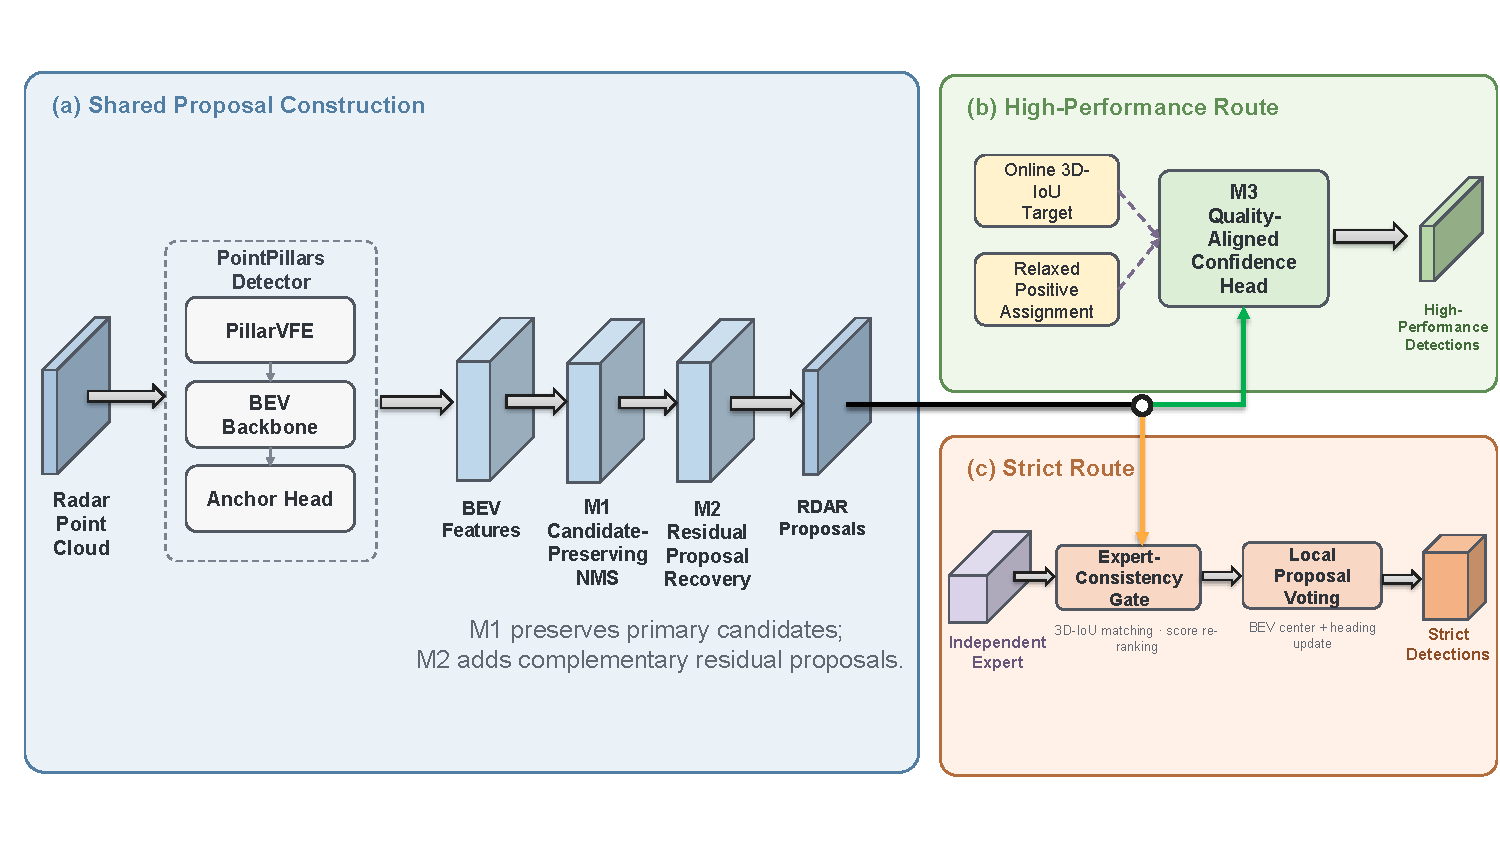
\includegraphics[width=\textwidth]{figures/fig1_framework_overview.pdf}
\caption{Overview of the proposal-refinement framework. PointPillars produces
BEV features; M1 preserves candidate proposals and M2 adds complementary
residual proposals to form the RDAR proposal stream. The high-performance
route combines the M3 quality-aligned confidence head with an online 3D-IoU
target and relaxed positive assignment. The strict route instead applies an
independently trained expert for consistency gating, followed by local
proposal voting.}
\label{fig:framework-overview}
\end{figure}

The seed-2028 progressive analysis follows the construction of the
high-performance route. By contrast, the formal strict comparison starts from
RDAR-compatible proposals and selects for positive differences in all 12
dataset--seed pairs. The two analyses therefore measure different operating
objectives.

\subsection{Candidate preservation and recovery}

\subsubsection{M1: candidate-preserving NMS}

The baseline configuration uses a score threshold of 0.10 and a very strict
NMS IoU threshold of 0.01. Such a setting produces a compact output, but it
can delete useful evidence before any complementary proposal is considered.
M1 lowers the score threshold to zero and increases the NMS threshold to 0.50.
The pre-NMS and post-NMS limits remain 4096 and 500, respectively. Thus M1
changes which boxes remain available, not the maximum reported proposal count.
The design intent is to delay irreversible deletion until complementary
evidence has been considered. M1 changes candidate availability rather than
detector capacity or the final proposal budget.

Let $\pi$ order boxes by score. Hard NMS accepts the highest remaining box and
removes a box $j$ whenever
\begin{equation}
\operatorname{IoU}_{3D}(\mathbf{b}_{\pi(i)},\mathbf{b}_j)>\tau_{\mathrm{nms}}.
\end{equation}
Increasing $\tau_{\mathrm{nms}}$ from 0.01 to 0.50 delays this deletion and
retains moderately overlapping alternatives. This resembles the preservation
motivation of Soft-NMS \cite{bodla2017softnms}, although our implementation
does not use continuous score decay. The retained alternatives become inputs
to recovery, quality-aware ranking, and voting.

Removing the initial score threshold does not mean every proposal is promoted
to a high-confidence detection. The post-NMS limit remains finite, subsequent
ranking uses the learned score, and residual additions in M2 are explicitly
capped below the positive primary-score range. M1 is therefore a candidate-
access operation: it creates the opportunity for later modules to use weak
boxes without treating them as correct detections.

\subsubsection{M2: residual proposal recovery}

M1 cannot restore a hypothesis that exists only in a complementary prediction
stream. M2 takes a primary set
$\mathcal{P}=\{(\mathbf{b}_i,s_i)\}$ and a residual set
$\mathcal{R}=\{(\mathbf{r}_j,t_j)\}$. Frame identifiers and ordering are
validated before fusion. The residual boxes are sorted by $t_j$, and only the
top $K_r=50$ are processed.

The design intent is conservative recovery. A residual may contribute geometry
when it supports a primary proposal, but its score must remain below the
primary lane so that complementary evidence cannot override a confident
primary prediction.

For each residual proposal, we find
\begin{equation}
i^\star(j)=\arg\max_i
\operatorname{IoU}_{3D}(\mathbf{r}_j,\mathbf{b}_i).
\end{equation}
When the best IoU is at least $\tau_r=0.10$, the residual and primary
geometries are combined using normalized score weights. For the six
non-angular box parameters,
\begin{equation}
\widetilde{\mathbf{b}}_{j,1:6} =
\frac{s_{i^\star}\mathbf{b}_{i^\star,1:6}
+ t_j\mathbf{r}_{j,1:6}}
{s_{i^\star}+t_j}.
\end{equation}
Heading is $\pi$-periodic for an oriented rectangular box. We therefore use
doubled-angle circular averaging:
\begin{equation}
\widetilde{\theta}_j=\frac{1}{2}\operatorname{atan2}
\left(
\sum_{k\in\{i^\star,j\}}w_k\sin 2\theta_k,
\sum_{k\in\{i^\star,j\}}w_k\cos 2\theta_k
\right).
\end{equation}
This avoids cancellation when equivalent headings fall on opposite sides of
the numerical angle boundary. If the best overlap is below 0.10, the residual
geometry is appended unchanged.

Recovered proposals are deliberately prevented from dominating the primary
ranking. Let $s_{\min}^{+}$ be the smallest positive primary score in the
evaluated prediction set and $t_{\max}$ the maximum residual score in the
frame. The assigned recovery score is
\begin{equation}
s_j^{\mathrm{rec}} =
\left(\frac{s_{\min}^{+}}{2}\right)
\left(0.5+0.5\frac{t_j}{\max(t_{\max},\epsilon)}\right),
\label{eq:recovery-score}
\end{equation}
where adjacency denotes multiplication and $\epsilon=10^{-12}$ prevents
division by zero. The factor in parentheses lies in $[0.5,1]$, so every
residual score is at most half the smallest positive primary score.

\subsection{Localization-quality-aware confidence (M3 branch)}

M3 is an accuracy-oriented comparison branch, not a component of the primary
expert-consistency endpoint. It is included because confidence ordering is a
separate design axis from expert agreement; reporting it separately prevents
the larger macro-AP gain from being mistaken for the main reliability claim.

Binary positive labels do not distinguish anchors by localization accuracy.
M3 replaces the positive classification target with an online 3D-IoU target.
For each positive anchor, the predicted residual and assigned regression
target are decoded into $\mathbf{b}_i$ and $\mathbf{g}_i$. Their aligned
quality is
\begin{equation}
q_i=\operatorname{IoU}_{3D}(\mathbf{b}_i,\mathbf{g}_i)\in[0,1].
\end{equation}
The IoU is detached from the classification graph, so the classification loss
does not back-propagate through the IoU operation into box regression.

Directly using $q_i$ can make a valid positive behave nearly like a negative
while the regressor is immature. We retain a residual objectness component:
\begin{equation}
\widehat q_i=\rho+(1-\rho)q_i^\gamma,
\qquad \rho=0.55,\quad \gamma=1.0.
\label{eq:quality-target}
\end{equation}
Negatives receive zero and ignored anchors are excluded. The parameter $\rho$
controls the minimum target for an assigned positive. At $\rho=1$, the target
reduces to binary objectness; at $\rho=0$, it is pure IoU quality. The selected
value retains both signals.

Let $z_i$ be the classification logit and $p_i=\sigma(z_i)$. The quality focal
term is
\begin{equation}
\mathcal{L}_{\mathrm{QF}} =
\frac{1}{N_+}\sum_{i\in\mathcal{C}}
\left|\widehat q_i-p_i\right|^\beta
\operatorname{BCEWithLogits}(z_i,\widehat q_i),
\qquad \beta=2,
\end{equation}
where the juxtaposition after the modulation factor denotes multiplication,
$\mathcal{C}$ is the set of cared anchors, and $N_+$ is the number of
positives, clipped below by one. This construction follows the general
quality-aware principle of Generalized Focal Loss
\cite{li2022gfl}, but uses online aligned 3D IoU and an explicit objectness
floor for sparse radar.

The full training loss is
\begin{equation}
\mathcal{L}=\mathcal{L}_{\mathrm{QF}}
+2\mathcal{L}_{\mathrm{box}}+0.2\mathcal{L}_{\mathrm{dir}}.
\end{equation}
M3 does not add a second inference branch. The original classification logit
is trained to express the combined objectness--quality target, leaving the
4.830 M parameter count unchanged. The M3-only control retains the
baseline assignment configuration and uses the candidate-preserving
post-processing settings. The separate high-performance route combines M3
with 0.50/0.35 positive/negative assignment thresholds and the
accuracy-oriented prior configuration.

The design intent is to make the ranking score reflect localization quality
without discarding objectness. The role of M3 is ranking: a well-localized proposal should receive a larger
target than a poorly localized proposal assigned to the same class. Better
ranking can improve which proposal survives NMS and where a detection appears
on the precision--recall curve. It does not guarantee that confidence is
calibrated in every sense, so ECE is measured independently in
Section~\ref{sec:calibration}.

\subsection{Expert-guided refinement}

The strict route applies two proposal-level operations to a primary RDAR set:
an expert-consistency quality gate and local box voting. The expert is a
stable BEV-gated detector with the same output parameterization. Its purpose is
not to replace the primary detector but to provide a second assessment of
whether a proposal is spatially supported. The strict route is selected by the
paired no-regression gate described below, not by the performance of a single
seed.

For reproducibility, the expert uses the same PointPillars-style radar input,
class definition, box coder, and seven-parameter output head as the primary
stream. Its configuration has a 64-channel PillarVFE, a 32-channel
DensityAwarePillarGate in the pillar backbone, and a 64-channel BEV scatter.
The BEV backbone uses three blocks with depths $[3,5,5]$, strides
$[2,2,2]$, filters $[64,128,256]$, and three 128-channel upsampling paths.
After concatenation, the expert applies a stable squeeze--excitation gate with
reduction 8 and an initial bounded residual scale of 0.1, followed by the
multi-scale BEV context module with hidden width 32, dilations $[1,2,4]$, and
initial residual scale 0.1. The gate is channel-wise: for BEV feature $x$ it
computes $x\mapsto x(1+r(2\sigma(g(\operatorname{GAP}(x)))-1))$, where $r$ is
a learned bounded scalar initialized to 0.1. At the pillar level, the density-aware gate
normalizes each pillar feature $p_i$, forms a scene context $c_i$ by averaging
normalized pillars from the same sample, and encodes the normalized point
count $d_i=\operatorname{clip}(\log(1+n_i)/\log(33),0,1)$. Specifically,
$p_i=\operatorname{LayerNorm}(p_i^{\rm raw})$, and $c_i$ is computed only
from pillars whose first coordinate in the voxel-coordinate tensor equals the
batch index of $i$; different batch samples therefore never share context.
If a sample has no occupied pillars, the module returns it unchanged. It then computes

\begin{equation}
z_i=2\,\sigma\!\left(W_2\,\operatorname{GELU}\!\left(W_1[p_i;c_i;d_i]\right)\right)-1,
\qquad p_i' = p_i\odot(1+r_p z_i),
\end{equation}

where $W_1,W_2$ are biased linear layers with the framework's default parameter
initialization, the hidden width is 32, and $r_p$ is a learned scalar
initialized to zero. The multi-scale
BEV context first reduces the concatenated BEV tensor to 32 channels, applies
depthwise $3\times3$ branches with dilations $1,2,4$, concatenates the branch
outputs, projects them back to the original channel count using a bias-free
$1\times1$ convolution followed by batch normalization, and adds the residual
$r_c h(x)$ with scalar $r_c=0.1$ at initialization. Each depthwise branch uses
its own shared reduced input but does not share branch weights. These definitions make
the expert modules explicit rather than relying only on YAML names. In the
released implementation these correspond to the classes
\texttt{DensityAwarePillarGate} and \texttt{MultiScaleBEVContext}; the stable
channel gate is \texttt{StableSEGate2D}. Their source files are
\texttt{density\_aware\_pillar\_gate.py} and
\texttt{base\_bev\_backbone.py} in the archived commit. The expert
is trained independently with the
same frozen split, augmentation policy, optimizer, 160-epoch schedule, and
checkpoint epoch as the paired primary configuration; no additional labels or
sensor inputs are used. The exact dataset-specific YAML files, checkpoint
paths, and commit are included in the reproducibility archive.
The fixed-expert checkpoint filenames, epoch, provenance paths, and SHA256
hashes are listed in
\texttt{expert\_checkpoint\_manifest\_20260730.md}.
For the fixed-expert factorial audit, the expert checkpoint is held fixed
within each conversion: seed 2027 is used for Astyx, TruckScenes, and
V2X-Radar-V, and seed 2028 is used for K-Radar, while the primary prediction
stream varies over seeds 2026, 2027, and 2028. This prevents the expert from
implicitly tracking the seed of each primary cell.

\subsubsection{Expert-consistency quality gate}

Let $\mathcal{E}=\{(\mathbf{e}_j,u_j)\}$ be the expert predictions. The final
$K_r=50$ entries of the combined primary set are reserved for residual
additions and are not gated. The gate is a support test rather than a second
detector decision: agreement raises a proposal's rank, while disagreement
lowers its rank without deleting the box. For every other primary proposal, the
best expert match is
\begin{equation}
j^\star(i)=\arg\max_j
\operatorname{IoU}_{3D}(\mathbf{b}_i,\mathbf{e}_j).
\end{equation}
If the maximum IoU $v_i$ is at least $\tau_e=0.30$, the score becomes
\begin{equation}
s'_i=s_i^{1-\alpha}u_{j^\star}^{\alpha}v_i^\eta,
\qquad \alpha=0.30,\quad \eta=0.25.
\label{eq:quality-gate}
\end{equation}
This geometric product requires agreement among primary confidence, expert
confidence, and overlap. The small IoU exponent avoids allowing modest
geometric noise to erase otherwise supported radar proposals. If $v_i<0.30$,
the proposal is retained but down-weighted:
\begin{equation}
s'_i=\kappa s_i,\qquad \kappa=0.50.
\end{equation}
Keeping unmatched proposals instead of deleting them preserves the conservative
character of the pipeline. The gate affects ranking but does not move a box.

\subsubsection{Local proposal voting}

The voting stage refines geometry using the gated scores. Its design intent is
to correct small center and heading errors while avoiding changes to box size,
which could create artificial IoU gains. For each primary box
$i$, a neighborhood is defined by
\begin{equation}
\mathcal{N}_i=\{j:
\operatorname{IoU}_{3D}(\mathbf{b}_i,\mathbf{b}_j)\geq\tau_v\},
\qquad \tau_v=0.24.
\end{equation}
If $\lvert\mathcal{N}_i\rvert\leq1$, the box is unchanged. Otherwise,
$w_j=\max(s'_j,10^{-8})$ and
\begin{equation}
\mathbf{c}_{i,1:6}=
\frac{\sum_{j\in\mathcal{N}_i}w_j\mathbf{b}_{j,1:6}}
{\sum_{j\in\mathcal{N}_i}w_j}
\end{equation}
defines the consensus geometry. Consensus heading is again calculated in
doubled-angle space. The strict \texttt{xy} mode updates only the BEV center:
\begin{equation}
\mathbf{b}'_{i,xy}=(1-\lambda)\mathbf{b}_{i,xy}
+\lambda\mathbf{c}_{i,xy},
\qquad \lambda=0.40.
\label{eq:voting}
\end{equation}
Heading is interpolated circularly with weights $1-\lambda$ and $\lambda$.
Height, center $z$, length, width, and height remain unchanged. Restricting the
update prevents the consensus from artificially shrinking or expanding boxes
to satisfy the evaluation threshold.

The IoU neighborhood threshold is lower than the 0.50 evaluation threshold.
This is intentional: multiple radar hypotheses for the same vehicle can have
modest 3D overlap because of height and dimension noise while still agreeing
in BEV. Threshold sensitivity is nevertheless evaluated over a closed grid
rather than justified only after observing the selected setting. The final 50
residual proposals remain outside the voting pool, ensuring that consistency
refinement cannot undo M2 by moving or suppressing the recovered tail.

The stages preserve a fixed division of responsibility. M1 determines which
primary candidates survive, and M2 adds complementary residual proposals. In
the strict route, expert consistency changes only the ranking of primary
proposals. Local voting then updates only the BEV center and heading of
supported primary boxes. Residual proposals never enter the gate or voting
pool, and voting does not change box dimensions.

\subsection{Operating routes and selection criteria}

The \emph{RDAR baseline} denotes M1 followed by M2 under the frozen recovery
protocol. The \emph{M3-only control} applies M3 and provides the
intermediate trainable comparison. The \emph{high-performance route} uses the
same quality-focal formulation with relaxed positive assignment and the
accuracy-oriented prior configuration. It is chosen by macro AP across the
four datasets. Its intended use is to show the performance available when
average accuracy is prioritized.

The \emph{strict route} applies the expert gate and local vote. Let
$A_{d,r}^{m}$ be AP for method $m$, dataset $d$, and seed $r$. A candidate is
strict only when
\begin{equation}
\Delta_{d,r}=A_{d,r}^{m}-A_{d,r}^{\mathrm{RDAR}}>0
\quad\forall(d,r)\in\mathcal{D}\times\mathcal{S},
\label{eq:strict-gate}
\end{equation}
where $\lvert\mathcal{D}\rvert=4$ and $\lvert\mathcal{S}\rvert=3$.
This definition contains no tolerance for a small negative difference. It is
stronger than requiring a positive macro mean, but remains bounded to the
tested data, splits, and seeds.

Selection by Eq.~\eqref{eq:strict-gate} is not a claim that the strict route
has the highest AP. Indeed, the high-performance route has a larger macro
mean. The two routes answer different engineering questions: whether a
configuration offers the largest average gain and whether it avoids a
regression in the available paired tests.

\tabref{tab:routes} lists the exact operations enabled by every reported
configuration. It should be consulted when comparing the M3-only control,
high-performance route, and strict route because they optimize different
objectives and are not successive aliases for one model. In particular,
relaxed positive assignment belongs to the high-performance route, whereas
expert gating and local voting define the strict route.

\begin{samepage}
\noindent\begin{minipage}{\textwidth}
\refstepcounter{table}\label{tab:routes}
\noindent\textbf{Table \thetable.} Definitions of the operating routes and
controls. M1 and M2 form the shared candidate-preserving proposal stream; the
remaining columns identify the additional scoring or refinement operations.\par
\vspace{2pt}
\scriptsize
\begin{tabularx}{\textwidth}{@{}
>{\raggedright\arraybackslash}X
>{\raggedright\arraybackslash}X
>{\raggedright\arraybackslash}X
>{\raggedright\arraybackslash}X
>{\raggedright\arraybackslash}X
>{\raggedright\arraybackslash}X@{}}
\toprule
Config\-uration & M1+M2 stream & M3 score & Expert gate & Local vote & Selection objective \\
\midrule
RDAR baseline & Yes & Binary objectness & No & No & Reference \\
M3-only control & Yes & IoU-aware quality & No & No & Isolate quality ranking \\
High-performance route & Yes & IoU-aware quality + relaxed assignment & No & No & Maximize macro AP \\
Strict route & Yes & RDAR score & Yes & Yes & Positive paired differences \\
\bottomrule
\end{tabularx}
\end{minipage}
\end{samepage}

\subsection{Algorithmic summary}

For clarity, the complete procedure is summarized below.
\begin{enumerate}[leftmargin=*,label=\textbf{Step \arabic*:}]
\item Encode the radar frame with PillarVFE, scatter pillar features to BEV,
and predict anchor classification, box residuals, and direction.
\item During M3 training, decode positive boxes, compute aligned 3D IoU, form
the soft target in Eq.~\eqref{eq:quality-target}, and optimize the combined
loss. The baseline route retains binary classification.
\item Apply candidate-preserving NMS with zero initial score threshold,
$\tau_{\mathrm{nms}}=0.50$, and a 500-box post-NMS limit.
\item Retain the top 50 complementary residual proposals. Fuse a residual box
with its best primary match when 3D IoU is at least 0.10; otherwise append it.
Assign the conservative score in Eq.~\eqref{eq:recovery-score}.
\item For the strict route, match each non-residual primary proposal to the
expert stream, apply Eq.~\eqref{eq:quality-gate}, and down-weight unmatched
boxes by 0.50.
\item Form local neighborhoods at $\tau_v=0.24$ and update BEV center and
heading using Eq.~\eqref{eq:voting}. Return the residual tail unchanged.
\item Rank the resulting predictions and evaluate them with the identical
AP$_{R40}$ implementation used for every compared method.
\end{enumerate}

\subsection{Training and implementation details}

Training uses the OpenPCDet codebase and an Adam one-cycle optimizer for 160
epochs. The frozen baseline configuration uses a per-GPU batch size of four,
initial learning rate 0.003, weight decay 0.01, momentum 0.9, one-cycle
momenta $[0.95,0.85]$, warm-up fraction 0.4, division factor 10, and gradient
norm clipping at 10. Random world flips, rotations in
$[-\pi/4,\pi/4]$, and scaling in $[0.95,1.05]$ are applied during training.
Ground-truth sampling is disabled in the frozen radar configuration used for
the controlled comparisons.

All models are trained independently with seeds 2026, 2027, and 2028. The
formal comparison uses the same data partitions, class definition, metric,
checkpoint epoch, and evaluation code for each paired method. Proposal-level
scripts validate frame order before combining prediction files. This check is
important because an apparently valid fusion between misaligned frame lists
could silently produce meaningless boxes.

The progressive construction study is intentionally narrower. It holds the
seed at 2028 and adds M1, M2, quality alignment, and the high-performance
calibration variant sequentially. It is used to identify the contribution
scale of the stages, not to establish that every intermediate module is
positive for all seeds. The formal strict result instead evaluates the final
strict route on all 12 paired cells.

Computational cost is reported in three parts. Trainable parameters distinguish
model capacity. A fixed profiler measures detector forward execution including
OpenPCDet post-processing but excluding AP computation and result
serialization. A separate timer measures only the local voting loop and
excludes prediction-file input/output. Keeping these measurements separate
prevents a fast detector result from hiding an expensive post-processing
stage.

\subsection{Implementation safeguards}

The implementation uses four safeguards that define the scope of the claim.
Prediction files must have identical frame order; residual scores are bounded
by Eq.~\eqref{eq:recovery-score} and kept in the final 50-entry tail, outside
the gate and voting pool; and residual fusion and voting use doubled-angle
averaging for the $\pi$-periodic heading. The strict vote updates only $x$,
$y$, and heading, while $z$, $l$, $w$, and $h$ remain unchanged. Finally, one
global threshold setting is used across all four datasets; dataset-specific
compensation screens are reported only as diagnostics. These constraints keep
the comparison auditable and prevent the reliability endpoint from becoming a
collection of independently tuned dataset-specific procedures.

\section{Experimental Protocol}

\subsection{Research questions}

We ask five questions. RQ1 tests whether the strict route improves RDAR in
every matched dataset--seed comparison. RQ2 isolates the contribution of each
component, and RQ3 examines sensitivity to expert and threshold selection.
RQ4 compares AP with calibration and controlled point loss. RQ5 reports the
computational cost of both routes.

\subsection{Datasets and protocol}

We evaluate radar-only car detection on four datasets. Astyx provides an
automotive radar point-cloud benchmark \cite{meyer2019astyx}. MAN TruckScenes
covers autonomous trucking scenes and a sensor geometry distinct from
passenger-car platforms \cite{fent2024truckscenes}.
For V2X-Radar-V, we use the vehicle-side subset of a cooperative 4D radar
collection. K-Radar contains 4D radar measurements acquired in varied weather
\cite{paek2022kradar,yang2024v2xradar}. The experiment records refer to the
frozen conversions as Astyx, TruckScenes-mini, V2X-Radar-V-400, and
K-Radar-400. We use shorter names in the text. The experiment package retains
the exact conversion names, configuration files, and frozen outputs.

The frozen splits contain 300/100 train/validation frames for Astyx and 320/80
for each remaining conversion, with 531, 3950, 268, and 198 validation car
instances, respectively. The records provide frame-level point-cloud,
calibration, image, and annotation fields but no scene or sequence identifiers.
We found no exact train--validation overlap in the available point-cloud IDs.
We also applied a conservative adjacency check: a symmetric $\pm1$ difference
in \texttt{point\_cloud.pc\_idx}. It flagged 82/100 Astyx, 4/80 TruckScenes,
1/80 V2X-Radar-V, and 80/80 K-Radar validation frames. The converted records
do not contain ordering metadata, so this check cannot establish temporal
adjacency. It also cannot rule out correlations from the same scene or
vehicle. Excluding all flagged frames would leave 18, 76, 79, and 0 validation
frames, making K-Radar AP impossible to estimate. Our evaluation is therefore
limited to the frozen frame-level protocol. We do not claim scene-disjoint,
vehicle-disjoint, cross-initialization, or deployment generalization. The
``mini'' and ``400'' suffixes name the conversion protocol, not new dataset
releases.

The primary metric is car AP$_{R40}$ at 0.50 3D IoU, evaluated with a common
implementation and class mapping. AP is reported on a 0--100 scale, so a
difference of 1.0 is one AP point. Because AP is computed over the complete
validation set and is not additive over frames, frame and instance counts
describe evaluation scope rather than define per-frame confidence intervals.
The paired and cluster-resampling summaries describe only these finite frozen
sets.

The formal experiment uses four datasets and three seeds (2026, 2027, and
2028). Each model is trained independently under the same schedule and
evaluated with the same class mapping and code. We report the mean and sample
standard deviation across seeds. For the strict route, comparisons are paired
within each seed. The primary detector and expert are trained independently,
but use the same data protocol and seed. This pairing makes individual
regressions visible without introducing a cross-seed difference. We examine
that issue separately by holding the expert fixed across seeds. This diagnostic
tests sensitivity, not initialization-independent robustness.

The main claims rely on the formal three-seed comparison. The seed-2028
progressive study is used only to examine the construction path. Calibration,
point dropout, threshold transfer, runtime, and qualitative cases probe model
behavior and practical limits.

\tabref{tab:datasets} summarizes the conversions, inputs, spatial ranges, and
training seeds. Acquisition settings differ, but the class mapping,
AP$_{R40}$ metric, 0.50 3D-IoU threshold, and paired-seed rule are shared.

\begin{samepage}
\noindent
\begin{minipage}{\textwidth}
\refstepcounter{table}\label{tab:datasets}
\noindent\textbf{Table \thetable.} Dataset scope and common protocol for the
formal four-dataset, three-seed evaluation.\par
\vspace{2pt}
\begingroup
\scriptsize
\setlength{\tabcolsep}{2pt}
\renewcommand{\arraystretch}{1.22}
\begin{tabularx}{\textwidth}{@{}
  >{\raggedright\arraybackslash}p{0.13\textwidth}
  >{\raggedright\arraybackslash}p{0.14\textwidth}
  >{\raggedright\arraybackslash}X
  >{\raggedright\arraybackslash}p{0.13\textwidth}
  >{\raggedright\arraybackslash}p{0.22\textwidth}
  >{\raggedright\arraybackslash}p{0.12\textwidth}@{}}
\toprule
Dataset & Frozen conversion & Platform or acquisition setting & Model input &
\shortstack{Spatial range\\$[x,y,z]$ (m)} & Formal seeds \\
\midrule
Astyx & Astyx & Automotive passenger-vehicle scenes & Radar point cloud &
$[0,60]\times[-25,25]\times[-3,2]$ & 2026, 2027, 2028 \\
MAN TruckScenes & TruckScenes-mini & Autonomous trucking scenes & Radar point cloud &
$[0,60]\times[-25,25]\times[-3,2]$ & 2026, 2027, 2028 \\
V2X-Radar-V & V2X-Radar-V-400 & Vehicle-side cooperative-perception subset &
4D radar point cloud & $[0,60]\times[-25,25]\times[-3,2]$ & 2026, 2027, 2028 \\
K-Radar & K-Radar-400 & Driving scenes under varied weather conditions &
4D radar point cloud & $[0,60]\times[-25,25]\times[-3,2]$ & 2026, 2027, 2028 \\
\bottomrule
\end{tabularx}
\endgroup
\vspace{2pt}
\parbox{\textwidth}{\scriptsize
All rows use the paper's frozen car-class mapping and are evaluated with
AP$_{R40}$ at a 3D-IoU match threshold of 0.50. Each method is trained
independently for the three listed seeds, and paired method--RDAR differences
are calculated within the same dataset and seed. The spatial range is the
common model input range recorded in the frozen configurations, not a claim
about the physical maximum range of each sensor.}
\end{minipage}
\end{samepage}

\subsection{Baselines and comparison routes}

The conventional PointPillars-style detector is the architectural reference.
RDAR, comprising M1 and M2, is the paired baseline for the formal comparison.
The M3-only control isolates M3, and the high-performance route combines
M3 with relaxed assignment and the accuracy-oriented prior. The strict route
adds expert-consistency score refinement and conditional geometry voting to
RDAR-compatible primary proposals. Frozen-output controls include standard box
voting, Gaussian Soft-NMS, and weighted box fusion. A gate--vote factorial
comparison and a fixed-expert audit are used to attribute the strict-route
effect.

\subsection{Metrics and statistical summaries}

For a ranked list at a fixed 3D-IoU match threshold, precision and recall after
the first $k$ predictions are
\begin{equation}
\operatorname{Prec}(k)=\frac{\operatorname{TP}(k)}
{\operatorname{TP}(k)+\operatorname{FP}(k)},\qquad
\operatorname{Rec}(k)=\frac{\operatorname{TP}(k)}
{\operatorname{TP}(k)+\operatorname{FN}(k)}.
\end{equation}
AP$_{R40}$ samples the interpolated precision envelope at 40 recall positions.
Because confidence determines the traversal order, M3 can change AP even when
the set of decoded boxes is similar. Because voting changes geometry, the
strict route can also change which predictions cross the 0.50 IoU matching
threshold.

The macro result for method $m$ is the unweighted average of the four
dataset-level seed means:
\begin{equation}
\overline A_{\mathrm{macro}}^m =
\frac{1}{4}\sum_{d\in\mathcal{D}}
\left(\frac{1}{3}\sum_{r\in\mathcal{S}} A_{d,r}^m\right).
\end{equation}
This choice gives each dataset equal influence regardless of the number of
frames or objects. It avoids allowing the largest validation partition to
dominate, but it does not imply equal operational importance.

Standard deviations describe variation across the three seeds; they are not
confidence intervals for dataset performance. For the strict comparison, we
report all 12 paired differences, their mean and median, a bootstrap interval,
and an exact sign test. We place greater weight on the effect sizes and the
smallest paired gain. Threshold selection and evaluation use the same
four-dataset protocol, so the result describes consistency within this
protocol rather than held-out performance. Resampling the four dataset means
gives a descriptive interval of [0.5464, 1.4834] AP.

\section{Results}
\label{sec:results}

\subsection{Main comparison}

\tabref{tab:main-results} compares the two operating endpoints with RDAR and
the M3-only control over three seeds. The high-performance route is evaluated
by macro AP and calibration, whereas the strict route is evaluated by its
paired AP difference from RDAR in each dataset--seed cell.

\begin{samepage}
\noindent
\begin{minipage}{\textwidth}
\refstepcounter{table}\label{tab:main-results}
\noindent\textbf{Table \thetable.} Main three-seed comparison of RDAR, the
M3-only control, the high-performance route, and the strict route.\par
\vspace{2pt}
\begingroup
\scriptsize
\setlength{\tabcolsep}{3pt}
\renewcommand{\arraystretch}{1.18}
\resizebox{\textwidth}{!}{%
\begin{tabular}{@{}lrrrrrrc@{}}
\toprule
Route & Astyx & TruckScenes & V2X-Radar-V & K-Radar & Macro &
$\Delta$Macro & \shortstack{Positive\\paired cells} \\
\midrule
RDAR & $32.8347\pm1.4689$ & $16.3671\pm1.7480$ &
$41.7029\pm1.1490$ & $50.5163\pm2.0546$ & 35.3552 & -- & -- \\
M3-only & $35.8438\pm1.0680$ & $16.9661\pm1.2785$ &
$\mathbf{44.4122\pm2.5011}$ & $57.6910\pm2.5304$ & 38.7283 & +3.3731 & 11/12 \\
High-performance & $\mathbf{36.9801\pm0.9748}$ & $16.8063\pm1.1764$ &
$44.3786\pm0.5122$ & $\mathbf{58.3208\pm1.6943}$ &
$\mathbf{39.1214}$ & $\mathbf{+3.7662}$ & 11/12 \\
Strict & $33.6898\pm1.7215$ & $\mathbf{17.2878\pm1.7127}$ &
$42.1245\pm1.0852$ & $52.2091\pm2.5654$ & 36.3278 & +0.9726 & \textbf{12/12} \\
\bottomrule
\end{tabular}}
\endgroup
\vspace{2pt}
\parbox{\textwidth}{\scriptsize
Values are AP$_{R40}$ mean $\pm$ sample standard deviation over seeds 2026,
2027, and 2028 at a 3D-IoU threshold of 0.50. Macro is the unweighted mean of
the four dataset means, and $\Delta$Macro is measured from RDAR. Bold values
mark the largest result in each dataset or aggregate column. ``Positive paired
cells'' counts the dataset--seed cells with an AP increase relative to RDAR.
The M3-only control and high-performance route correspond to the frozen
quality-aware and accuracy-oriented configurations described above.}
\end{minipage}
\end{samepage}

The strict route raises macro AP from 35.3552 to 36.3278 (+0.9726). It also
improves all 12 matched dataset--seed cells. The high-performance route reaches
39.1214 macro AP (+3.7662), with its largest gain on K-Radar. Its only decrease
is on TruckScenes at seed 2027, from 18.3845 to 17.1075 AP. The M3-only control
reaches 38.7283 macro AP and has the same negative cell. The paired differences
are plotted in \figref{fig:paired-differences} and listed in
\tabref{tab:paired-results}.

\begin{figure}[htbp]
\centering
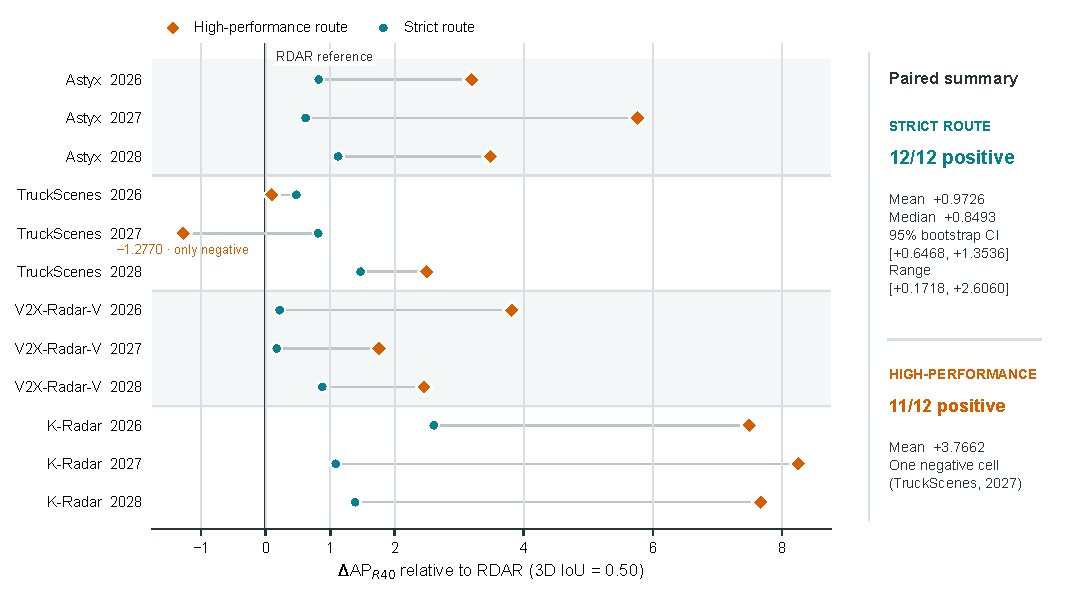
\includegraphics[width=\textwidth]{figures/fig3_paired_differences.pdf}
\caption{Paired AP differences relative to RDAR across the four datasets and
three seeds. The strict route remains positive in every tested dataset--seed
cell, whereas the high-performance route contains one negative cell.}
\label{fig:paired-differences}
\end{figure}

\tabref{tab:paired-results} gives the complete matched-seed audit for the
strict route.

\begin{samepage}
\noindent
\begin{minipage}{\textwidth}
\refstepcounter{table}\label{tab:paired-results}
\noindent\textbf{Table \thetable.} Complete matched-seed reliability audit for
the strict route.\par
\vspace{2pt}
\begingroup
\scriptsize
\setlength{\tabcolsep}{4pt}
\renewcommand{\arraystretch}{1.14}
\begin{tabularx}{\textwidth}{@{}Xrrrr@{}}
\toprule
Dataset & Seed & RDAR AP & Strict AP & $\Delta$AP \\
\midrule
Astyx & 2026 & 32.7281 & 33.5503 & +0.8222 \\
Astyx & 2027 & 31.4220 & 32.0422 & +0.6202 \\
Astyx & 2028 & 34.3540 & 35.4768 & +1.1228 \\
\addlinespace
TruckScenes & 2026 & 15.4127 & 15.8892 & +0.4765 \\
TruckScenes & 2027 & 18.3845 & 19.1980 & +0.8135 \\
TruckScenes & 2028 & 15.3041 & 16.7762 & +1.4721 \\
\addlinespace
V2X-Radar-V & 2026 & 40.7802 & 40.9969 & +0.2167 \\
V2X-Radar-V & 2027 & 42.9899 & 43.1617 & \textbf{+0.1718} \\
V2X-Radar-V & 2028 & 41.3385 & 42.2148 & +0.8763 \\
\addlinespace
K-Radar & 2026 & 51.3450 & 53.9510 & \textbf{+2.6060} \\
K-Radar & 2027 & 48.1767 & 49.2631 & +1.0864 \\
K-Radar & 2028 & 52.0271 & 53.4132 & +1.3861 \\
\bottomrule
\end{tabularx}
\endgroup
\vspace{2pt}
\parbox{\textwidth}{\scriptsize
Strict AP is the RDAR value plus the frozen matched difference for the strict
route. Across the 12 cells, the mean, median, minimum, and maximum $\Delta$AP
are 0.9726, 0.8493, 0.1718, and 2.6060. The nonparametric bootstrap 95\%
interval for the mean is [0.6468, 1.3536]. The exact sign test gives one-sided
$p=0.000244$ and two-sided $p=0.000488$; these tests are auxiliary summaries
for the finite evaluated cells.}
\end{minipage}
\end{samepage}

All paired differences are positive. Removing the largest gain does not change
this result. The smallest margin is 0.1718 AP on V2X-Radar-V at seed 2027.
The table note and experimental protocol give the remaining effect-size and
uncertainty summaries.

\subsection{Component and Control Analysis}

We applied three fixed-parameter controls to the same frozen RDAR predictions.
They use the same AP code and require neither expert predictions nor additional
labels. In \tabref{tab:postprocessing-controls}, standard box voting is
positive for all three seeds on Astyx and V2X-Radar-V. Gaussian Soft-NMS and
weighted box fusion do not meet this criterion on any dataset. None matches
the strict route across all four datasets.

\begin{samepage}
\noindent\begin{minipage}{\textwidth}
\refstepcounter{table}\label{tab:postprocessing-controls}
\noindent\textbf{Table \thetable.} Three-seed controls for generic proposal
post-processing. Values are mean AP differences relative to RDAR.\par
\vspace{2pt}\scriptsize
\begin{tabularx}{\textwidth}{@{}Xrrrrc@{}}
\toprule
Control & Astyx & TruckScenes & V2X-Radar-V & K-Radar &
\shortstack{Datasets positive\\in all three seeds} \\
\midrule
Standard box voting & +0.4723 & -0.0831 & +0.5342 & +0.0097 & 2/4 \\
Gaussian Soft-NMS ($\sigma=0.5$) & -0.1831 & +0.0909 & -0.2098 & +0.0196 & 0/4 \\
Weighted box fusion (IoU $=0.5$) & -0.0118 & -0.1305 & -0.2474 & -0.1896 & 0/4 \\
Strict route & +0.8551 & +0.9207 & +0.4216 & +1.6928 & 4/4 \\
\bottomrule
\end{tabularx}
\vspace{2pt}\parbox{\textwidth}{\scriptsize
All methods start from the same frozen RDAR prediction files and evaluator;
control parameters were fixed before three-seed aggregation.}
\end{minipage}\end{samepage}

Across the 12 primary cells, vote-only changes mean AP by $-0.0274$ and
improves 6/12 cells. We then fixed one expert checkpoint within each dataset
instead of matching the seed. Under this test, gate-only improves 11/12 cells,
and gate-plus-vote improves 10/12. Both regressions occur on Astyx. The matched
strict result is narrowest on V2X-Radar-V: its mean gain is 0.4216 AP, with two
seed-level gains below 0.22 AP.

\subsubsection{Progressive construction}

\figref{fig:progressive-analysis} follows the seed-2028 construction path on
the four datasets. M1 has its clearest effect on Astyx, whereas M2 changes the
result only slightly. M3 produces the largest macro step, especially on
K-Radar. This analysis uses one seed.

\begin{figure}[htbp]
\centering

\includegraphics[width=\textwidth]{figures/fig4_progressive_seed2028.pdf}
\caption{Progressive construction on seed 2028. M1 and M2 preserve and recover
candidate evidence, while M3 supplies the dominant accuracy-oriented gain; the
plot is a mechanism analysis for one seed rather than a multi-seed monotonicity
claim.}
\label{fig:progressive-analysis}
\end{figure}

Relative to the preceding configuration, M1 adds 1.7483 macro AP and M2 adds
0.0169. M3 raises macro AP from 35.7559 to 39.1379. The corresponding gains
are 2.6778 AP on Astyx, 2.1489 on TruckScenes, 1.2594 on V2X-Radar-V, and
7.4416 on K-Radar. The final accuracy-oriented adjustment adds 0.6446 AP.

\subsection{Robustness and Threshold Sensitivity}
\label{sec:calibration}

\figref{fig:diagnostics} summarizes calibration, controlled point loss, voting
thresholds, and the number of positive paired cells.

\begin{figure}[htbp]
\centering

\includegraphics[width=\textwidth]{figures/fig5_diagnostics.pdf}
\caption{Diagnostic and boundary analyses. Panels compare calibration,
controlled point loss, voting thresholds, and the number of positive paired
cells across the reported routes.}
\label{fig:diagnostics}
\end{figure}

ECE compares mean confidence with empirical correctness within confidence
bins \cite{guo2017calibration}. The high-performance route lowers ECE in all
12 three-seed comparisons, with a mean reduction of 0.0504. At seed 2028, the
reductions are 0.0749 on Astyx, 0.0407 on TruckScenes, 0.0354 on V2X-Radar-V,
and 0.0845 on K-Radar. M3-only gives the lowest ECE on V2X-Radar-V; the
high-performance route is lowest on the other datasets. In contrast, the
strict route increases ECE in all 12 comparisons by 0.0270 on average.

The range-bin audit gives the strict route 26 wins, 13 ties, and 9 losses. Its
sparsity audit gives 18 wins, 19 ties, 8 losses, and 3 missing cells. The
high-performance route records 17 range-bin wins, 10 ties, and 21 losses.
The bin-level counts include both improvements and regressions.

\subsubsection{Point-dropout stress test}

We dropped radar points before voxelization with a fixed seed of 3407. No model
was retrained or adapted. The high-performance route remains ahead at 10\%,
20\%, and 30\% dropout. Its changes from the clean checkpoint are $+0.1242$,
$-1.2030$, and $-1.7970$ AP. The corresponding RDAR changes are $-2.6651$,
$-3.9114$, and $-3.3868$, a mean difference in degradation of 2.3624 AP.

Across datasets and dropout rates, the high-performance route exceeds RDAR in
11/12 cells. The exception is TruckScenes at 30\%: 11.9555 versus 12.0161 AP,
a difference of $-0.0606$. Adding an exploratory vote fixes this cell but
reduces the original result in 8/12 cells, so we leave the endpoint unchanged.

\subsubsection{Voting-threshold sensitivity}

\figref{fig:diagnostics}(c,d) shows the complete grid over voting IoU and
strength. Three neighboring settings also remain positive in all 12
dataset--seed pairs: $(0.22,0.40)$ reaches 36.1364 macro AP, $(0.24,0.45)$
reaches 36.2165, and $(0.24,0.50)$ reaches 36.0479. The highest grid value,
36.3393 at $(0.25,0.40)$, is positive in 11 of 12 pairs. The selected
$(0.24,0.40)$ setting reaches 36.3278 macro AP and remains the best setting
under the 12-of-12 criterion.

\subsubsection{Held-out threshold transfer}

For leave-one-dataset-out transfer, the conservative screen keeps settings with
nine positive training differences and then selects the highest mean. The
unconstrained screen selects by training mean alone. Without further tuning,
the conservative rule gives positive held-out means for all four datasets and
11/12 positive seed differences. The unconstrained rule yields one negative
cell: $-0.2945$ AP on V2X-Radar-V at seed 2027. This audit is separate from the
formal threshold-selected result.

\subsection{Qualitative Cases}

\figref{fig:qualitative-cases} compares RDAR and strict-route boxes for three
selected borderline misses. The examples show how center and heading updates
can cross the 0.50 matching threshold without changing box dimensions. They do
not indicate how often this occurs.

\begin{figure}[H]
\centering
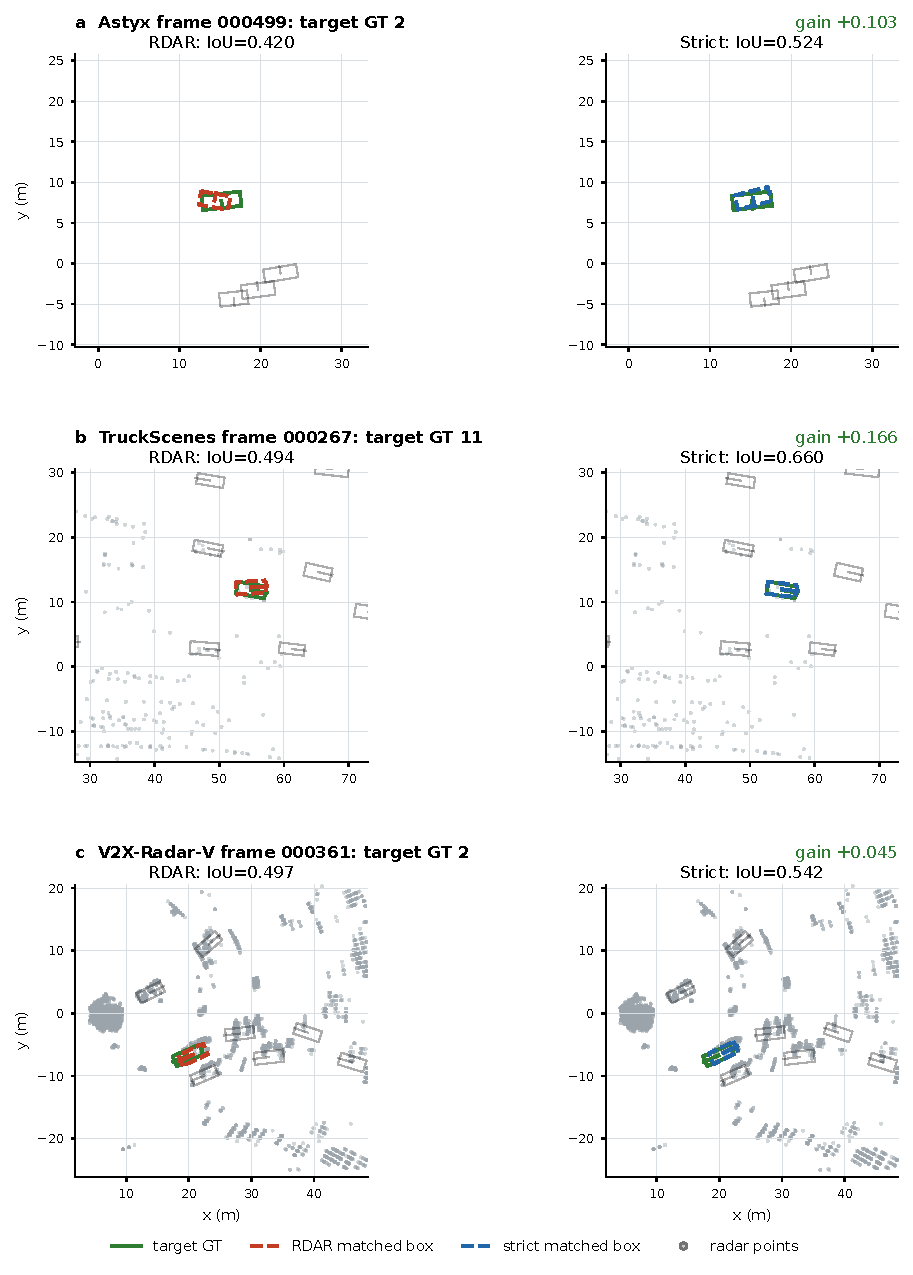
\includegraphics[width=0.98\textwidth]{figures/fig6_qualitative_bev.pdf}
\caption{Qualitative BEV cases comparing RDAR and the strict route against the
same ground-truth targets. The constrained update changes center and heading
while keeping box dimensions fixed.}
\label{fig:qualitative-cases}
\end{figure}

Conditional voting raises IoU from 0.4203 to 0.5235 in Astyx frame 000499. It
raises IoU from 0.4940 to 0.6599 in TruckScenes frame 000267 and from 0.4970 to
0.5420 in V2X-Radar-V frame 000361. In each case, the restricted $xy$ and
heading update turns a borderline localization into a valid match without
resizing the box.

\subsection{Computational Cost}

\tabref{tab:efficiency} reports parameter counts and timing measurements. M3
changes the training target rather than network width, so the M3-only and
high-performance detectors retain the RDAR parameter count. Voting adds no
trainable parameters, but it adds proposal-refinement time. We report detector
forward time, isolated voting time, and endpoint time separately.

\begin{samepage}
\noindent\begin{minipage}{\textwidth}
\refstepcounter{table}\label{tab:efficiency}
\noindent\textbf{Table \thetable.} Component-level parameter and runtime
profile on an NVIDIA GeForce RTX 3090.\par\vspace{2pt}\scriptsize
\begin{tabularx}{\textwidth}{@{}XrX@{}}
\toprule
Configuration & Parameters & Parameter interpretation \\
\midrule
RDAR detector & 4.830 M & Primary detector and frozen internal baseline \\
Quality-aligned detector & 4.830 M & M3 changes supervision, not network width \\
High-performance detector & 4.830 M & Separate trained accuracy-oriented endpoint \\
Stable expert detector & 4.868 M & Auxiliary detector used by the strict route \\
Strict voting operation & +0 & Proposal-level operation with no trainable weights \\
\bottomrule
\end{tabularx}
\vspace{3pt}
\begin{tabularx}{\textwidth}{@{}Xrrrr@{}}
\toprule
Profiled stage & Astyx & TruckScenes & V2X-Radar-V & K-Radar \\
\midrule
RDAR detector forward & $4.740\pm0.297$ & $3.851\pm0.311$ & $4.834\pm1.092$ & $5.887\pm2.409$ \\
High-performance detector forward & $8.263\pm1.163$ & $7.880\pm1.257$ & $8.124\pm1.334$ & $8.601\pm1.471$ \\
Strict voting loop & $22.7095\pm0.1031$ & $22.0086\pm0.1826$ & $22.5393\pm0.0471$ & $22.8485\pm0.1735$ \\
\bottomrule
\end{tabularx}
\vspace{2pt}\parbox{\textwidth}{\scriptsize
Hardware: NVIDIA GeForce RTX 3090. Detector-forward profiling uses batch size
4 and excludes AP evaluation, result serialization, expert inference, and
prediction-file I/O. Independently profiled rows must not be summed as an
end-to-end strict-route latency.}
\end{minipage}\end{samepage}

Both M3-based detectors have 4.830 M parameters, the same as RDAR. The expert
used by the strict route has 4.868 M parameters, and voting has no trainable
weights. On the RTX 3090, the high-performance detector remains below 9 ms per
frame but is slower than RDAR. The isolated 500-proposal voting loop takes
about 22--23 ms. It constructs 3D IoUs on the GPU, then visits the local
neighborhoods in a Python loop.

For completeness, an exploratory batch-1 profile runs primary forward, expert
forward, and post-processing in one process on an RTX 4080 SUPER. Mean times are 16.08 ms
on Astyx, 23.11 ms on TruckScenes, and 21.62 ms on V2X-Radar-V. These values
correspond to 62.2, 43.3, and 46.3 Hz, with 197--201 MB peak allocated memory.
The sampled Astyx frames return 20--27 proposals, unlike the 500-proposal
RTX 3090 component profile, so the two sets of timings are not combined. In a
separate scaling test, voting takes
1.5--1.6 ms for 50 proposals and 9.7--10.1 ms for 500. Peak incremental
allocation is approximately 6.7 MB.

\section{Discussion}

No single route dominates across all criteria. The high-performance route has
the larger mean AP gain and better calibration, but one matched comparison is
negative. The strict route improves all 12 dataset--seed cells, with a smaller
mean gain and poorer calibration. In practice, the choice is between maximizing
average detection quality and avoiding a regression under the present protocol.

\subsection{Mechanism and Relation to Prior Work}

Candidate preservation leaves alternative hypotheses available after the first
suppression step, while residual recovery restores proposals that would
otherwise disappear. In the seed-2028 construction, most of the macro-AP
increase comes from M3. Localization-aware ranking is therefore the main
contributor in this run. Since the progressive experiment uses only one seed,
the same ordering cannot be assumed across runs.

The controls help explain why the strict route behaves differently from generic
post-processing. Vote-only improves 6 of the 12 primary cells. Neither fixed
Soft-NMS nor weighted box fusion produces three positive seeds on any dataset.
When one expert checkpoint is fixed within each dataset, gate-only is positive
in 11/12 cells and gate-plus-vote in 10/12. These results place most of the
stability benefit in the independent expert check, with voting playing a more
selective role. They do not isolate the gate completely because the fixed-expert
and matched-expert protocols differ.

The expert check also separates the strict route from existing post-processing
methods. Soft-NMS adjusts scores from proposal overlap, whereas weighted box
fusion averages coordinates using detector confidence
\cite{bodla2017softnms,solovyev2021wbf}. Here, an independently trained expert
determines whether a primary proposal can be re-ranked or updated. M3 acts
earlier by aligning the ranking score with localization quality, an idea shared
with IoU-aware confidence methods \cite{jiang2018iounet,li2022gfl}. Our
experiments examine how these two operations interact on a fixed
PointPillars-style backbone; they do not show that either class of method can be
replaced.

\subsection{Operational Trade-Offs and Boundaries}

AP consistency and calibration move in opposite directions. The
high-performance route lowers ECE in all 12 comparisons, whereas the strict
route raises it in all 12. Strict-route scores should therefore be recalibrated
before they are used as probabilities for risk-sensitive thresholding. The
high-performance route is the more natural choice when ranking and confidence
quality matter together.

Robustness is similarly uneven. The range and sparsity audits contain both wins
and losses, and TruckScenes regresses at 30\% point dropout. Point density,
return geometry, or the localization errors presented to the expert may account
for some of this variation, but the current audits do not separate these
factors. The gains are consequently specific to the tested datasets and
operating regimes.

The computational profiles add another practical constraint. The
high-performance detector retains the RDAR parameter count but has higher
forward latency. The strict route also requires expert inference, and its
500-proposal Python voting loop takes about 22--23 ms on the RTX 3090. Because
the exploratory RTX 4080 SUPER profile uses different proposal counts, it is not
directly comparable with the component-level RTX 3090 measurements. A deployment
decision must account for calibration, the cost of a regression, and the
available latency budget.

\subsection{Limitations and future work}

The conclusions are bounded by radar-only car detection, four dataset
conversions, three seeds, and one PointPillars-style detector. The smallest
strict gain is 0.1718 AP, and the voting threshold is selected within the same
evaluation protocol. Leave-one-dataset-out selection reduces this dependence
but still produces one negative held-out seed. The frame manifests do not allow
a scene-disjoint audit, and the progressive construction uses only one seed.
The qualitative examples are selected successful corrections, not an estimate
of how often such cases occur.

Another gap is the lack of a protocol-matched comparison with recent public
radar-only detectors. Published scores based on different dataset conversions,
spatial ranges, and evaluators cannot be inserted fairly into the present table.
The most useful next tests are development-set threshold selection, scene-aware
splits, additional detector families and classes, and reproduced public
baselines under the same evaluator. Post-hoc calibration of the strict route
and a batched or sparse-neighbourhood voting implementation would address the
two main deployment costs identified here.

\section{Conclusion}

We introduced a proposal-level refinement framework for radar-only 3D car
detection that leaves the detector backbone unchanged. It retains alternative
candidates, uses localization quality in proposal ranking, and checks proposed
updates against an independently trained expert. Over four dataset conversions
and three seeds, the strict route improved AP in all 12 matched dataset--seed
comparisons, with an average gain of 0.9726 AP. The high-performance route achieved
the larger macro-AP increase, from 35.3552 to 39.1214, and lowered ECE in every
comparison, but it regressed on one TruckScenes seed.

Neither route was better on every criterion. The strict route was more
consistent in matched AP, but its ECE increased in all 12 comparisons and it
added the cost of expert inference and local voting. The high-performance route
was less consistent across seeds, although it gave stronger average accuracy
and calibration. These findings are confined to radar-only car detection with
four dataset conversions, three seeds, and a PointPillars-style backbone.
Further evaluation should choose thresholds on a development set and reproduce
recent methods under the same evaluator. Tests on other detectors and classes,
together with a faster voting implementation, would show how well the findings
carry beyond the current setting.

\authorcontributions{Zixuan Liu: Conceptualization, Methodology, Software,
Validation, Formal analysis, Investigation, Data curation, Writing--original
draft, and Visualization. Wei Xiong: Supervision, Project administration,
Funding acquisition, and Writing--review and editing. All authors have read and
agreed to the published version of the manuscript.}

\funding{This work was supported in part by the National Natural Science
Foundation of China under Grant 62202148, in part by the Natural Science
Foundation of Hubei Province under Grants 2022CFB908 and 2019CFB530, and in
part by the China Scholarship Council under Grant 201808420418.}

\institutionalreview{Not applicable.}

\informedconsent{Not applicable.}

\dataavailability{The paper uses four radar datasets and frozen experimental
outputs already recorded in the project workspace. Astyx, MAN TruckScenes,
V2X-Radar-V, and K-Radar are available from their original providers subject
to their respective access and license terms. Derived experimental
configurations, result summaries, manuscript sources, and reproducibility
materials supporting the findings are publicly available at the GitHub
repository
\href{https://github.com/niubisile-wq/sparse-radar-proposal-reliability}{github.com/niubisile-wq/sparse-radar-proposal-reliability}
and archived at Zenodo
(\href{https://doi.org/10.5281/zenodo.21696781}{DOI:
10.5281/zenodo.21696781}). The original datasets remain subject to the access
and licence terms of their providers; raw datasets and model checkpoints are
not redistributed in the repository.}

\conflictsofinterest{The authors declare that they have no known competing
financial interests or personal relationships that could have appeared to
influence the work reported in this paper.}

\begin{adjustwidth}{-\extralength}{0cm}
\reftitle{References}
\begin{thebibliography}{99}

\bibitem{qi2017pointnet}
C.~R. Qi, H. Su, K. Mo, and L.~J. Guibas,
\emph{PointNet: Deep Learning on Point Sets for 3D Classification and
Segmentation}, in: Proc. IEEE Conf. Computer Vision and Pattern Recognition
(CVPR), 2017, pp. 77--85.
\url{https://doi.org/10.1109/CVPR.2017.16}.

\bibitem{qi2017pointnetpp}
C.~R. Qi, L. Yi, H. Su, and L.~J. Guibas,
\emph{PointNet++: Deep Hierarchical Feature Learning on Point Sets in a Metric
Space}, in: Advances in Neural Information Processing Systems 30, 2017,
pp. 5099--5108.

\bibitem{zhou2018voxelnet}
Y. Zhou and O. Tuzel,
\emph{VoxelNet: End-to-End Learning for Point Cloud Based 3D Object
Detection}, in: Proc. IEEE/CVF Conf. Computer Vision and Pattern Recognition
(CVPR), 2018, pp. 4490--4499.
\url{https://doi.org/10.1109/CVPR.2018.00472}.

\bibitem{yan2018second}
Y. Yan, Y. Mao, and B. Li,
\emph{SECOND: Sparsely Embedded Convolutional Detection},
Sensors 18(10) (2018) 3337.
\url{https://doi.org/10.3390/s18103337}.

\bibitem{lang2019pointpillars}
A.~H. Lang, S. Vora, H. Caesar, L. Zhou, J. Yang, and O. Beijbom,
\emph{PointPillars: Fast Encoders for Object Detection from Point Clouds},
in: Proc. IEEE/CVF Conf. Computer Vision and Pattern Recognition (CVPR),
2019, pp. 12689--12697.
\url{https://doi.org/10.1109/CVPR.2019.01298}.

\bibitem{shi2019pointrcnn}
S. Shi, X. Wang, and H. Li,
\emph{PointRCNN: 3D Object Proposal Generation and Detection from Point
Cloud}, in: Proc. IEEE/CVF Conf. Computer Vision and Pattern Recognition
(CVPR), 2019, pp. 770--779.
\url{https://doi.org/10.1109/CVPR.2019.00086}.

\bibitem{shi2020pvrcnn}
S. Shi, C. Guo, L. Jiang, Z. Wang, J. Shi, X. Wang, and H. Li,
\emph{PV-RCNN: Point-Voxel Feature Set Abstraction for 3D Object Detection},
in: Proc. IEEE/CVF Conf. Computer Vision and Pattern Recognition (CVPR),
2020, pp. 10526--10535.
\url{https://doi.org/10.1109/CVPR42600.2020.01054}.

\bibitem{qi2019votenet}
C.~R. Qi, O. Litany, K. He, and L.~J. Guibas,
\emph{Deep Hough Voting for 3D Object Detection in Point Clouds},
in: Proc. IEEE/CVF Int. Conf. Computer Vision (ICCV), 2019,
pp. 9277--9286.
\url{https://doi.org/10.1109/ICCV.2019.00937}.

\bibitem{yin2021centerpoint}
T. Yin, X. Zhou, and P. Kr\"ahenb\"uhl,
\emph{Center-Based 3D Object Detection and Tracking},
in: Proc. IEEE/CVF Conf. Computer Vision and Pattern Recognition (CVPR),
2021, pp. 11784--11793.
\url{https://doi.org/10.1109/CVPR46437.2021.01161}.

\bibitem{ren2017fasterrcnn}
S. Ren, K. He, R. Girshick, and J. Sun,
\emph{Faster R-CNN: Towards Real-Time Object Detection with Region Proposal
Networks}, IEEE Trans. Pattern Anal. Mach. Intell. 39(6) (2017) 1137--1149.
\url{https://doi.org/10.1109/TPAMI.2016.2577031}.

\bibitem{lin2017focal}
T.-Y. Lin, P. Goyal, R. Girshick, K. He, and P. Doll\'ar,
\emph{Focal Loss for Dense Object Detection},
in: Proc. IEEE Int. Conf. Computer Vision (ICCV), 2017, pp. 2980--2988.
\url{https://doi.org/10.1109/ICCV.2017.324}.

\bibitem{tian2019fcos}
Z. Tian, C. Shen, H. Chen, and T. He,
\emph{FCOS: Fully Convolutional One-Stage Object Detection},
in: Proc. IEEE/CVF Int. Conf. Computer Vision (ICCV), 2019,
pp. 9626--9635.
\url{https://doi.org/10.1109/ICCV.2019.00972}.

\bibitem{zhang2020atss}
S. Zhang, C. Chi, Y. Yao, Z. Lei, and S.~Z. Li,
\emph{Bridging the Gap Between Anchor-Based and Anchor-Free Detection via
Adaptive Training Sample Selection}, in: Proc. IEEE/CVF Conf. Computer Vision
and Pattern Recognition (CVPR), 2020, pp. 9756--9765.
\url{https://doi.org/10.1109/CVPR42600.2020.00978}.

\bibitem{li2022gfl}
X. Li, C. Lv, W. Wang, G. Li, L. Yang, and J. Yang,
\emph{Generalized Focal Loss: Towards Efficient Representation Learning for
Dense Object Detection}, IEEE Trans. Pattern Anal. Mach. Intell. (2022) 1--14.
\url{https://doi.org/10.1109/TPAMI.2022.3180392}.

\bibitem{zhang2021varifocalnet}
H. Zhang, Y. Wang, F. Dayoub, and N. S\"underhauf,
\emph{VarifocalNet: An IoU-Aware Dense Object Detector},
in: Proc. IEEE/CVF Conf. Computer Vision and Pattern Recognition (CVPR),
2021, pp. 8510--8519.
\url{https://doi.org/10.1109/CVPR46437.2021.00841}.

\bibitem{jiang2018iounet}
B. Jiang, R. Luo, J. Mao, T. Xiao, and Y. Jiang,
\emph{Acquisition of Localization Confidence for Accurate Object Detection},
in: European Conf. Computer Vision (ECCV), 2018, pp. 784--799.
\url{https://doi.org/10.1007/978-3-030-01264-9_48}.

\bibitem{cai2018cascadercnn}
Z. Cai and N. Vasconcelos,
\emph{Cascade R-CNN: Delving into High Quality Object Detection},
in: Proc. IEEE/CVF Conf. Computer Vision and Pattern Recognition (CVPR),
2018, pp. 6154--6162.
\url{https://doi.org/10.1109/CVPR.2018.00644}.

\bibitem{bodla2017softnms}
N. Bodla, B. Singh, R. Chellappa, and L.~S. Davis,
\emph{Soft-NMS---Improving Object Detection with One Line of Code},
in: Proc. IEEE Int. Conf. Computer Vision (ICCV), 2017, pp. 5562--5570.
\url{https://doi.org/10.1109/ICCV.2017.593}.

\bibitem{sun2021sparsercnn}
P. Sun, R. Zhang, Y. Jiang, T. Kong, C. Xu, W. Zhan, M. Tomizuka, L. Li,
Z. Yuan, C. Wang, and P. Luo,
\emph{Sparse R-CNN: End-to-End Object Detection with Learnable Proposals},
in: Proc. IEEE/CVF Conf. Computer Vision and Pattern Recognition (CVPR),
2021, pp. 14454--14463.
\url{https://doi.org/10.1109/CVPR46437.2021.01422}.

\bibitem{graham2018submanifold}
B. Graham, M. Engelcke, and L. van der Maaten,
\emph{3D Semantic Segmentation with Submanifold Sparse Convolutional
Networks}, in: Proc. IEEE/CVF Conf. Computer Vision and Pattern Recognition
(CVPR), 2018, pp. 9224--9232.
\url{https://doi.org/10.1109/CVPR.2018.00961}.

\bibitem{wang2021rodnet}
Y. Wang, Z. Jiang, X. Gao, J.-N. Hwang, G. Xing, and H. Liu,
\emph{RODNet: Radar Object Detection Using Cross-Modal Supervision},
in: IEEE Winter Conf. Applications of Computer Vision (WACV), 2021,
pp. 504--513.
\url{https://doi.org/10.1109/WACV48630.2021.00055}.

\bibitem{patel2019radarspectra}
K. Patel, K. Rambach, T. Visentin, D. Rusev, M. Pfeiffer, and B. Yang,
\emph{Deep Learning-Based Object Classification on Automotive Radar
Spectra}, in: IEEE Radar Conf. (RadarConf), 2019, pp. 1--6.
\url{https://doi.org/10.1109/RADAR.2019.8835775}.

\bibitem{meyer2019astyx}
M. Meyer and G. Kuschk,
\emph{Automotive Radar Dataset for Deep Learning Based 3D Object Detection},
in: 16th European Radar Conf. (EuRAD), 2019, pp. 129--132.

\bibitem{fent2024truckscenes}
F. Fent, F. Kuttenreich, F. Ruch, F. Rizwin, S. Juergens, L. Lechermann,
C. Nissler, A. Perl, U. Voll, M. Yan, and M. Lienkamp,
\emph{MAN TruckScenes: A Multimodal Dataset for Autonomous Trucking in
Diverse Conditions}, in: Advances in Neural Information Processing Systems
37, 2024, pp. 62062--62082.
\url{https://doi.org/10.52202/079017-1982}.

\bibitem{paek2022kradar}
D.-H. Paek, S.-H. Kong, and K.~T. Wijaya,
\emph{K-Radar: 4D Radar Object Detection for Autonomous Driving in Various
Weather Conditions}, in: Advances in Neural Information Processing Systems
35, 2022, pp. 3819--3829.
\url{https://doi.org/10.52202/068431-0276}.

\bibitem{paek2023enhancedkradar}
D.-H. Paek, S.-H. Kong, and K.~T. Wijaya,
\emph{Enhanced K-Radar: Optimal Density Reduction to Improve Detection
Performance and Accessibility of 4D Radar Tensor-Based Object Detection},
in: IEEE Intelligent Vehicles Symposium (IV), 2023, pp. 1--6.
\url{https://doi.org/10.1109/IV55152.2023.10186820}.

\bibitem{palffy2022viewofdelft}
A. Palffy, E. Pool, S. Baratam, J.~F.~P. Kooij, and D.~M. Gavrila,
\emph{Multi-Class Road User Detection with 3+1D Radar in the View-of-Delft
Dataset}, IEEE Robot. Autom. Lett. 7(2) (2022) 4961--4968.
\url{https://doi.org/10.1109/LRA.2022.3147324}.

\bibitem{zheng2022tj4dradset}
L. Zheng, Z. Ma, X. Zhu, B. Tan, S. Li, K. Long, W. Sun, S. Chen, L. Zhang,
M. Wan, L. Huang, and J. Bai,
\emph{TJ4DRadSet: A 4D Radar Dataset for Autonomous Driving},
in: IEEE 25th Int. Conf. Intelligent Transportation Systems (ITSC), 2022,
pp. 493--498.
\url{https://doi.org/10.1109/ITSC55140.2022.9922539}.

\bibitem{yang2024v2xradar}
L. Yang, X. Zhang, J. Li, C. Wang, Z. Song, T. Zhao, Z. Song, L. Wang,
M. Zhou, Y. Shen, K. Wu, and C. Lv,
\emph{V2X-Radar: A Multi-Modal Dataset with 4D Radar for Cooperative
Perception}, arXiv:2411.10962, 2024.
\url{https://doi.org/10.48550/arXiv.2411.10962}.

\bibitem{long2023radiant}
Y. Long, A. Kumar, D. Morris, X. Liu, M. Castro, and P. Chakravarty,
\emph{RADIANT: Radar-Image Association Network for 3D Object Detection},
Proc. AAAI Conf. Artificial Intelligence 37(2) (2023) 1808--1816.
\url{https://doi.org/10.1609/aaai.v37i2.25270}.

\bibitem{nobis2021radarvoxelfusion}
F. Nobis, E. Shafiei, P. Karle, J. Betz, and M. Lienkamp,
\emph{Radar Voxel Fusion for 3D Object Detection},
Applied Sciences 11(12) (2021) 5598.
\url{https://doi.org/10.3390/app11125598}.

\bibitem{vora2020pointpainting}
S. Vora, A.~H. Lang, B. Helou, and O. Beijbom,
\emph{PointPainting: Sequential Fusion for 3D Object Detection},
in: Proc. IEEE/CVF Conf. Computer Vision and Pattern Recognition (CVPR),
2020, pp. 4603--4611.
\url{https://doi.org/10.1109/CVPR42600.2020.00466}.

\bibitem{montiel2024pointcloudpainting}
J. Montiel-Mar\'in, A. Llamazares, and M. Antunes,
\emph{Point Cloud Painting for 3D Object Detection with Camera and Automotive
3+1D Radar Fusion}, Sensors 24(4) (2024) 1244.
\url{https://doi.org/10.3390/s24041244}.

\bibitem{deng2024crossmodal}
J. Deng, G. Chan, H. Zhong, and C.~X. Lu,
\emph{Robust 3D Object Detection from LiDAR-Radar Point Clouds via
Cross-Modal Feature Augmentation}, in: IEEE Int. Conf. Robotics and
Automation (ICRA), 2024, pp. 6585--6591.
\url{https://doi.org/10.1109/ICRA57147.2024.10610775}.

\bibitem{zhang2024contrastiveradar}
C. Decourt, R. VanRullen, D. Salle, and T. Oberlin,
\emph{Leveraging Self-Supervised Instance Contrastive Learning for Radar
Object Detection}, arXiv:2402.08427, 2024.
\url{https://doi.org/10.48550/arXiv.2402.08427}.

\bibitem{kong2025rtnhplus}
S.-H. Kong, D.-H. Paek, and S. Lee,
\emph{RTNH+: Enhanced 4D Radar Object Detection Network Using Two-Level
Preprocessing and Vertical Encoding},
IEEE Trans. Intell. Veh. 10(2) (2025) 1427--1440.
\url{https://doi.org/10.1109/TIV.2024.3428696}.

\bibitem{song2026radarrepresentations}
S.-H. Song, D.-H. Paek, M.-Q. Dao, E. Malis, and S.-H. Kong,
\emph{Enhanced 3-D Object Detection via Diverse Feature Representations of
4-D Radar Tensor},
IEEE Sensors J. 26(5) (2026) 7242--7252.
\url{https://doi.org/10.1109/JSEN.2026.3652543}.

\bibitem{nabati2021centerfusion}
R. Nabati and H. Qi,
\emph{CenterFusion: Center-Based Radar and Camera Fusion for 3D Object
Detection},
in: IEEE/CVF Winter Conf. Applications of Computer Vision (WACV), 2021,
pp. 1526--1535.
\url{https://doi.org/10.1109/WACV48630.2021.00157}.

\bibitem{piergiovanni2021fourDnet}
A.~J. Piergiovanni, V. Casser, M.~S. Ryoo, and A. Angelova,
\emph{4D-Net for Learned Multi-Modal Alignment},
in: Proc. IEEE/CVF Int. Conf. Computer Vision (ICCV), 2021,
pp. 15415--15425.
\url{https://doi.org/10.1109/ICCV48922.2021.01515}.

\bibitem{feng2021tood}
C. Feng, Y. Zhong, Y. Gao, M.~R. Scott, and W. Huang,
\emph{TOOD: Task-Aligned One-Stage Object Detection},
in: Proc. IEEE/CVF Int. Conf. Computer Vision (ICCV), 2021,
pp. 3490--3499.
\url{https://doi.org/10.1109/ICCV48922.2021.00349}.

\bibitem{hosang2017learnnms}
J. Hosang, R. Benenson, and B. Schiele,
\emph{Learning Non-Maximum Suppression},
in: Proc. IEEE Conf. Computer Vision and Pattern Recognition (CVPR), 2017,
pp. 6469--6477.
\url{https://doi.org/10.1109/CVPR.2017.685}.

\bibitem{solovyev2021wbf}
R.~A. Solovyev, W. Wang, and T. Gabruseva,
\emph{Weighted Boxes Fusion: Ensembling Boxes from Different Object Detection
Models},
Image Vis. Comput. 107 (2021) 104117.
\url{https://doi.org/10.1016/j.imavis.2021.104117}.

\bibitem{kuppers2020detectioncalibration}
F. K\"uppers, J. Kronenberger, A. Shantia, and A. Haselhoff,
\emph{Multivariate Confidence Calibration for Object Detection},
in: Proc. IEEE/CVF Conf. Computer Vision and Pattern Recognition Workshops
(CVPRW), 2020, pp. 326--327.
\url{https://openaccess.thecvf.com/content_CVPRW_2020/html/w20/Kuppers_Multivariate_Confidence_Calibration_for_Object_Detection_CVPRW_2020_paper.html}.

\bibitem{pathiraja2023mccl}
B. Pathiraja, M. Gunawardhana, and M.~H. Khan,
\emph{Multiclass Confidence and Localization Calibration for Object
Detection},
in: Proc. IEEE/CVF Conf. Computer Vision and Pattern Recognition (CVPR),
2023, pp. 19734--19743.
\url{https://openaccess.thecvf.com/content/CVPR2023/html/Pathiraja_Multiclass_Confidence_and_Localization_Calibration_for_Object_Detection_CVPR_2023_paper.html}.

\bibitem{guo2017calibration}
C. Guo, G. Pleiss, Y. Sun, and K.~Q. Weinberger,
\emph{On Calibration of Modern Neural Networks},
in: Proc. 34th Int. Conf. Machine Learning, PMLR 70, 2017,
pp. 1321--1330.
\url{https://proceedings.mlr.press/v70/guo17a.html}.

\end{thebibliography}

\end{adjustwidth}

\end{document}
